% !TeX program = xelatex
%==============================================================
%  Python金融数据分析 · 第7章 数据输入输出
%  基于《Python金融大数据分析（第2版）》第9章内容改编
%  授课对象：本科金融系学生（已学完第2-6章）
%  编译：xelatex chapter7.tex（编译两遍）
%==============================================================
\documentclass[9pt]{ctexbeamer}

%%%%-----导入宏包-----%%%%
\usepackage{style/shubeamer}   % SHU 主题（配色、帧标题、页脚、Python代码样式）
\usepackage{amsmath,amsfonts,amssymb,bm}
\usepackage{graphicx,hyperref,url}
\usepackage{subcaption}
\usepackage{booktabs}
\usepackage[super,square]{natbib}
\usepackage{wrapfig}          % 文字绕排
\usepackage{calligra}         % 结尾页花体字

%%%%-----设置字体-----%%%%
\setmainfont{CMU Serif}
\setsansfont{CMU Sans Serif}

%%%%-----常用自定义颜色（正文可直接使用）-----%%%%
\definecolor{nvidia}{RGB}{102,156,28}
\definecolor{red}{RGB}{184,13,73}
\definecolor{orange}{RGB}{242,151,36}
\definecolor{darkteal}{RGB}{43,106,108}
\definecolor{darkblue}{RGB}{4,37,58}

%%%%-----每节开始时自动显示当前节目录-----%%%%
\AtBeginSection[]
{
	\begin{frame}<beamer>
		\frametitle{\textbf{目录}}
		\textbf{\tableofcontents[currentsection]}
	\end{frame}
}

%%%%-----设定图片存放路径-----%%%%
\graphicspath{{figures/}}

%%%%-----首页信息设置-----%%%%
\AtBeginDocument{%
	%%%%----短标题[显示在页脚]{封面标题}
	\title[Python金融数据分析 · 第7章]{\fontsize{16pt}{22pt}\selectfont {Python金融数据分析}}
	%%%%----副标题（本章主题）
	\subtitle{\fontsize{9pt}{14pt}\selectfont \textit{第7章\quad 数据输入输出}}
	%%%%----个人信息
	\author[王伟冠, 吕文俊]{%
		\begin{tabular}{ll}%
			主讲人： & 王伟冠, 吕文俊\tabularnewline%
			院\quad 系： & 经济学院金融系\tabularnewline
		\end{tabular}
	}
	%%%%----机构信息
	\institute[SHU]{上海大学}
	%%%%----日期信息
	\date[\today]{\today}}

%%%%-----数学宏（向量、矩阵、算子等，见 style/macros.tex）-----%%%%
\input{style/macros.tex}


\begin{document}

%% 封面
\begin{frame}
	\titlepage
\end{frame}

%% 目录页
\section*{目录}
\begin{frame}
	\frametitle{\textbf{目录}}
	\textbf{\tableofcontents}
\end{frame}


\section{从同一张表认识文件格式}

\begin{frame}{本章学习路线}
\begin{enumerate}
\item 观察同一套虚拟行情：不同文件如何表达同一份数据？
\item 制作虚拟行情：CSV、Excel、Parquet 三种版本。
\item 按格式学习操作：类型、分块、嵌套、工作表、选列。
\item 先验证读回结果，再比较文件体积与读取耗时。
\item 理解 Parquet 的列式存储，并用选列实验检查效果。
\end{enumerate}
\begin{block}{本章产物}
配套 Notebook 生成可打开的样本文件与实验结果；最后用真实行情完成“读入 $\to$ 计算 $\to$ 保存”。
\end{block}
\end{frame}



\begin{frame}{三种格式：分别为谁服务？}
\small
\begin{tabular}{p{1.5cm}p{3.5cm}p{4.5cm}}
\toprule
格式 & 组织方式 & 常见任务与操作重点 \\
\midrule
CSV & 分隔符文本，一张平面表 & 软件间交换；编码、类型、分块 \\
Excel & 工作簿中的多个工作表 & 人工整理和报告；选表、选列 \\
Parquet & 带模式信息的列式二进制 & 分析中间表；类型、压缩、按列读取 \\
\bottomrule
\end{tabular}
\begin{block}{课堂观察}
CSV 用记事本看内容；Excel 用表格软件看工作表；Parquet 用程序看模式和数据，不用文本编辑器解释二进制。
\end{block}
\end{frame}



\begin{frame}{实验数据：先小样本，再同源大表}
\begin{itemize}
\item 全章格式示例使用同一套行情，先查看前 6 行理解字段。
\item 虚拟行情：固定随机种子 7；每行是一条分钟观测。
\item 8 列：日期、代码、市场、价格、成交量、买价、卖价、评分。
\item 代码含前导零，市场含中文；评分每隔 17 行缺失一次。
\item 同一个 DataFrame 写出三种格式，全部不额外保存索引。
\end{itemize}
\begin{block}{文件直接放在 data 中}
\texttt{data/quotes.csv / .xlsx / .parquet}：同一份 20,000 行数据。\\
用 \texttt{head(6)} 查看小样本，不额外建目录。\\
数据仅为教学模拟，日期序列并非真实交易日历。
\end{block}
\end{frame}

\begin{frame}[fragile]{先制作文件，再开始读取实验}
\begin{lstlisting}
# Notebook 已设置 CHAPTER，并导入 sys
sys.path.insert(0, str(CHAPTER / "scripts"))
from prepare_data import prepare
quotes, DATA = prepare(20_000)
quotes.head(6)
\end{lstlisting}
\begin{itemize}
\item \texttt{scripts/prepare\_data.py} 包含生成规则和三种写法。
\item 每次从同一张表写出全部文件；生成、写入不进入读取计时。
\item 所需 pandas、numpy、openpyxl、pyarrow 使用课程环境。
\item 也可在课前运行脚本；课堂直接查看生成文件。
\end{itemize}
\end{frame}

\begin{frame}[fragile]{open + with：查看同一份行情文本}
\begin{lstlisting}
# DATA 在数据准备步骤中设置；不另造一份示例数据
with open(DATA / "quotes.csv", encoding="utf-8") as f:
    for _ in range(7):  # 表头 + 前 6 行
        print(f.readline().rstrip())
\end{lstlisting}
\begin{itemize}
\item 第一行是列名，后面每行是一条行情记录。
\item \texttt{with} 自动关闭文件；中文文本明确使用 UTF-8。
\item \texttt{r} 读取（默认），\texttt{w} 覆盖，\texttt{a} 追加。
\item 接下来仍读取这个文件，用 pandas 还原为 DataFrame。
\end{itemize}
\end{frame}

\begin{frame}{同一份数据：文本与表格预览}
\centering
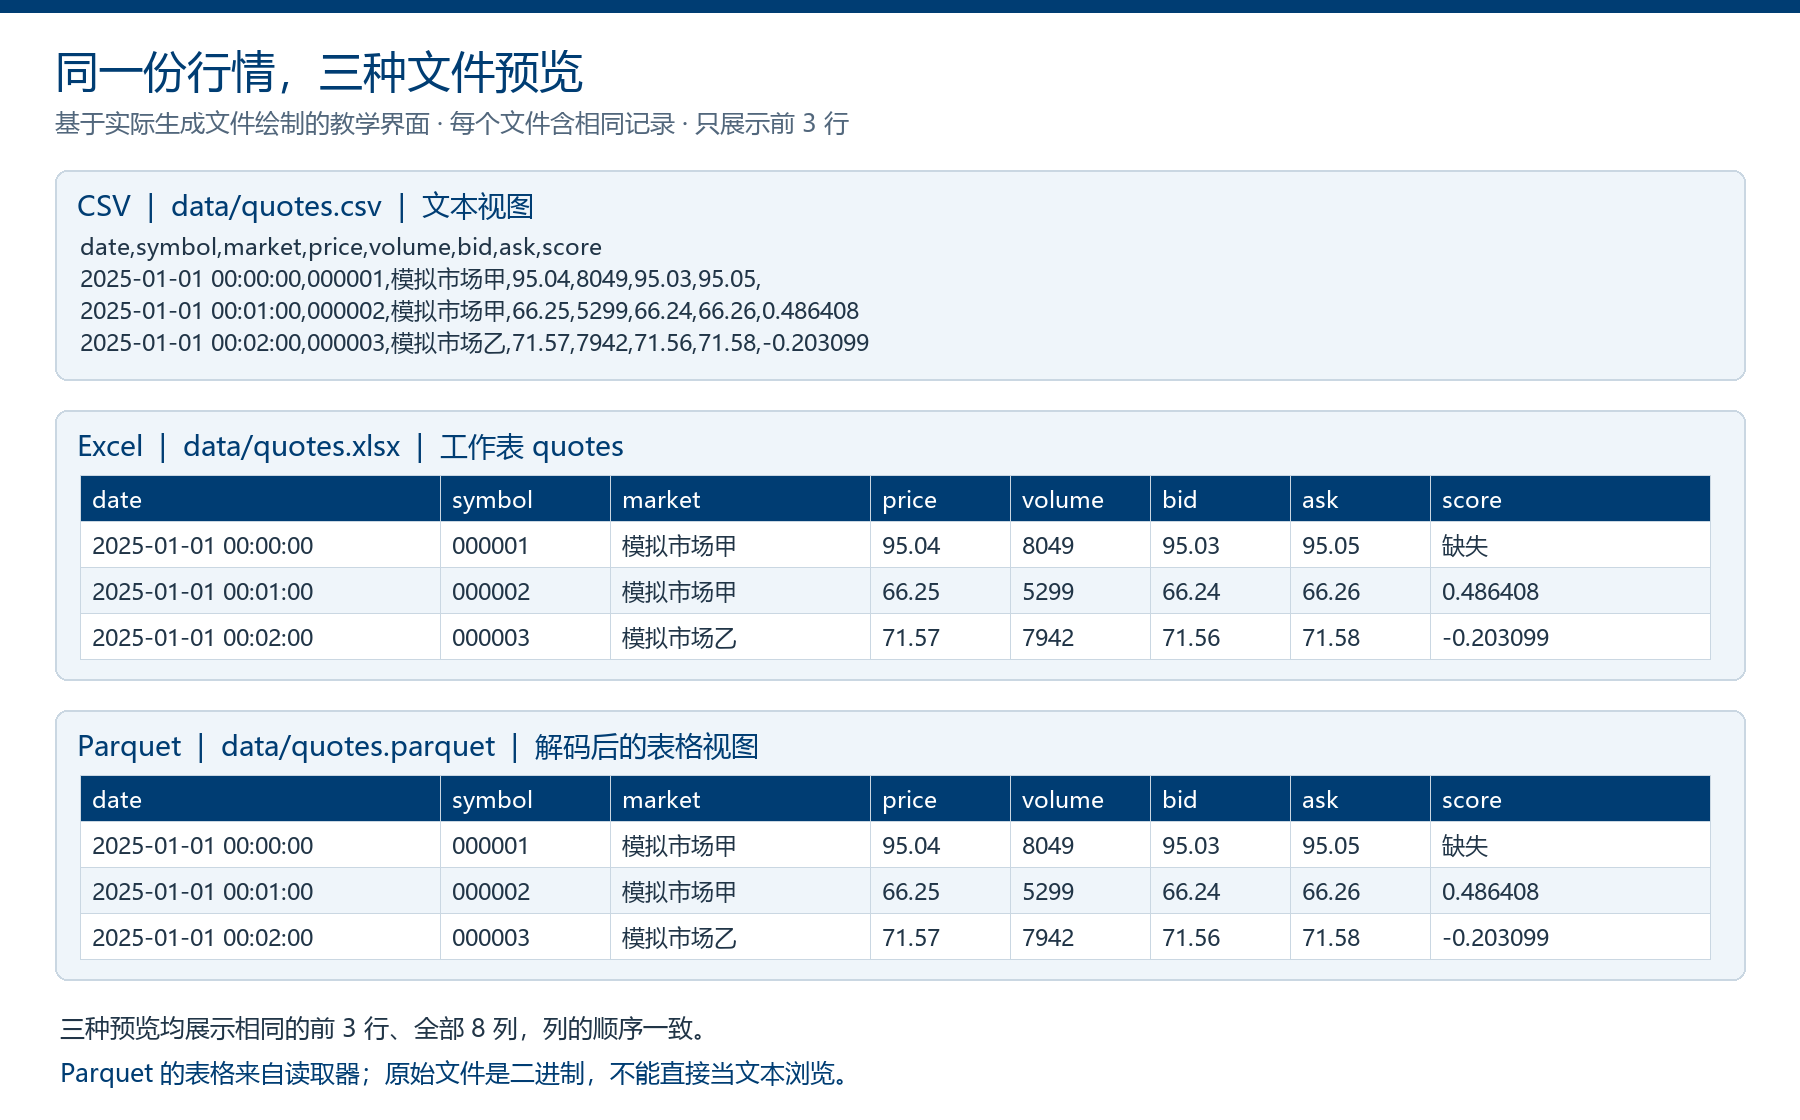
\includegraphics[width=\textwidth,height=.76\textheight,keepaspectratio]{formats_preview.png}
\end{frame}

\section{按格式学习操作特点}

\begin{frame}[fragile]{CSV：明确代码与日期的类型}
\begin{lstlisting}
quotes.to_csv(DATA / "quotes.csv", index=False,
              encoding="utf-8")
back = pd.read_csv(DATA / "quotes.csv",
                   dtype={"symbol": str},
                   parse_dates=["date"], encoding="utf-8")
\end{lstlisting}
\begin{itemize}
\item CSV 不保存 pandas 模式：\texttt{000001} 可能被推断为整数 1。
\item \texttt{dtype} 指定代码为字符串；\texttt{parse\_dates} 解析日期。
\item \texttt{sep} 指定分隔符，\texttt{na\_values} 约定缺失标记。
\item \texttt{index=False} 不写索引；如果日期在索引中，应明确保留它。
\end{itemize}
\end{frame}

\begin{frame}[fragile]{CSV：选列与分块是两种不同操作}
\begin{lstlisting}
small = pd.read_csv(DATA / "quotes.csv",
                    usecols=["price", "volume"])
total = 0
for chunk in pd.read_csv(DATA / "quotes.csv",
                         usecols=["volume"], chunksize=5000):
    total += chunk["volume"].sum()
assert total == quotes["volume"].sum()
\end{lstlisting}
\begin{itemize}
\item \texttt{usecols}：少构造几列，但仍需扫描 CSV 文本。
\item \texttt{chunksize}：每次处理部分行，适合求和、计数等任务。
\item 将全部块重新拼接，仍会回到整表占用内存的情况。
\item 字段内也可能有逗号或换行，不要用简单字符串切分替代解析器。
\end{itemize}
\end{frame}

\begin{frame}[fragile]{Excel：一个 Writer，多个工作表}
\begin{lstlisting}
summary = quotes.groupby("symbol", as_index=False)["volume"].sum()
with pd.ExcelWriter(DATA / "report.xlsx",
                     engine="openpyxl") as writer:
    quotes.head(6).to_excel(writer, sheet_name="行情", index=False)
    summary.to_excel(writer, sheet_name="汇总", index=False)
back = pd.read_excel(DATA / "report.xlsx",
                     sheet_name="汇总", dtype={"symbol": str})
\end{lstlisting}
\begin{alertblock}{不是连续对同一路径写两次}
两次独立的 \texttt{to\_excel("report.xlsx")} 默认会重建文件，前一个工作表会被覆盖。
\end{alertblock}
\end{frame}

\begin{frame}{Excel：给人阅读时的优势与边界}
\begin{itemize}
\item \texttt{sheet\_name} 选工作表，\texttt{usecols} 选列。
\item 用 \texttt{ExcelFile.sheet\_names} 查看工作簿中的表名。
\item \texttt{.xlsx} 的表格读取在本章明确使用 openpyxl 引擎。
\item pandas 读写数据表，不负责完整保留原工作簿的图表、样式与公式计算行为。
\item 大表反复分析前应实测：工作簿结构的解析本身有开销。
\end{itemize}
\begin{block}{交付习惯}
给同事阅读的汇总表可以用 Excel；计算中间表可以另存 Parquet。
\end{block}
\end{frame}

\section{Parquet 与列式存储}

\begin{frame}{从三列小表理解“按列放在一起”}
\begin{center}
\begin{tabular}{ccc}
\toprule
代码 & 价格 & 成交量 \\
\midrule
000001 & 12.5 & 200 \\
000002 & 20.0 & 300 \\
000003 & 18.2 & 100 \\
\bottomrule
\end{tabular}
\end{center}
\begin{block}{按行组织的示意}
\texttt{[000001, 12.5, 200] [000002, 20.0, 300] [000003, 18.2, 100]}
\end{block}
\begin{exampleblock}{按列组织的示意}
代码：\texttt{[000001, 000002, 000003]}\\
价格：\texttt{[12.5, 20.0, 18.2]}\quad 成交量：\texttt{[200, 300, 100]}
\end{exampleblock}
只计算平均价格时，列式布局有机会少读另外两列。
\end{frame}

\begin{frame}{Parquet 文件内部：行组与列块}
\centering
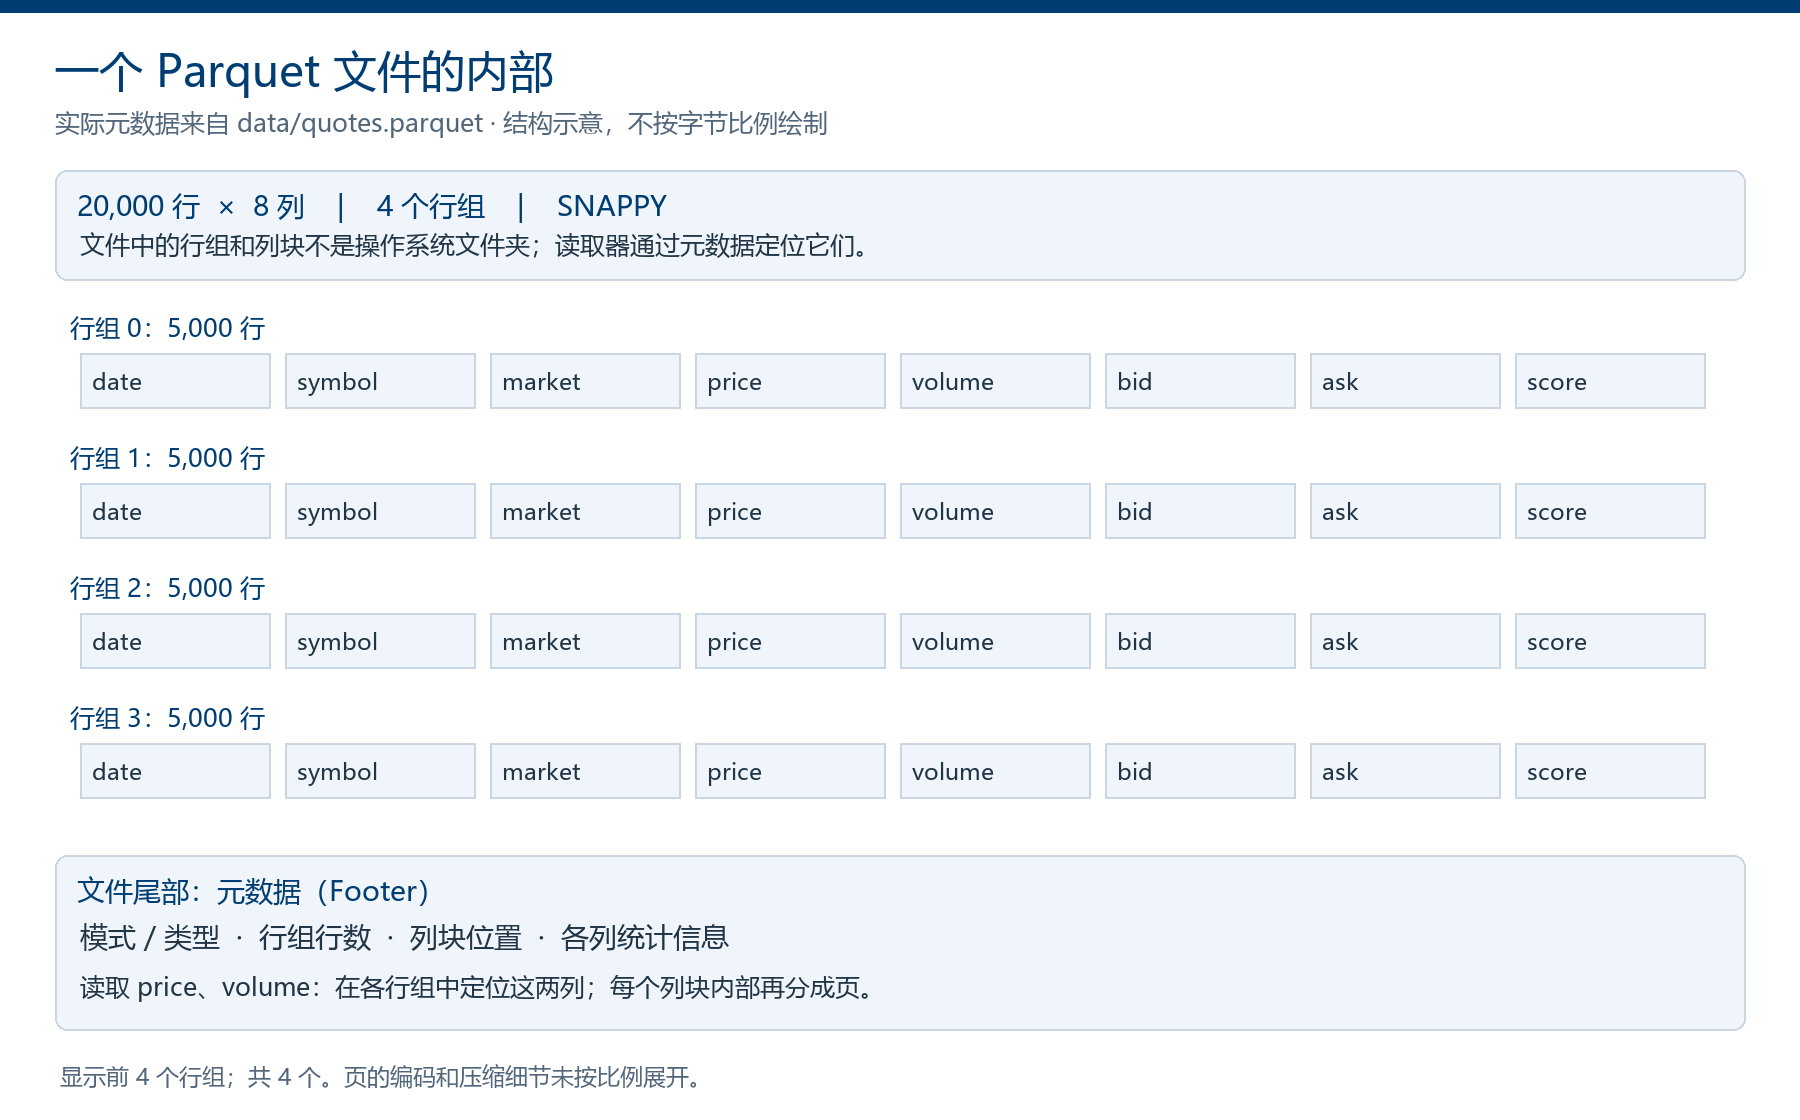
\includegraphics[width=\textwidth,height=.78\textheight,keepaspectratio]{parquet_layout.png}
\end{frame}

\begin{frame}{Parquet 数据集：分区目录与文件安排}
\centering
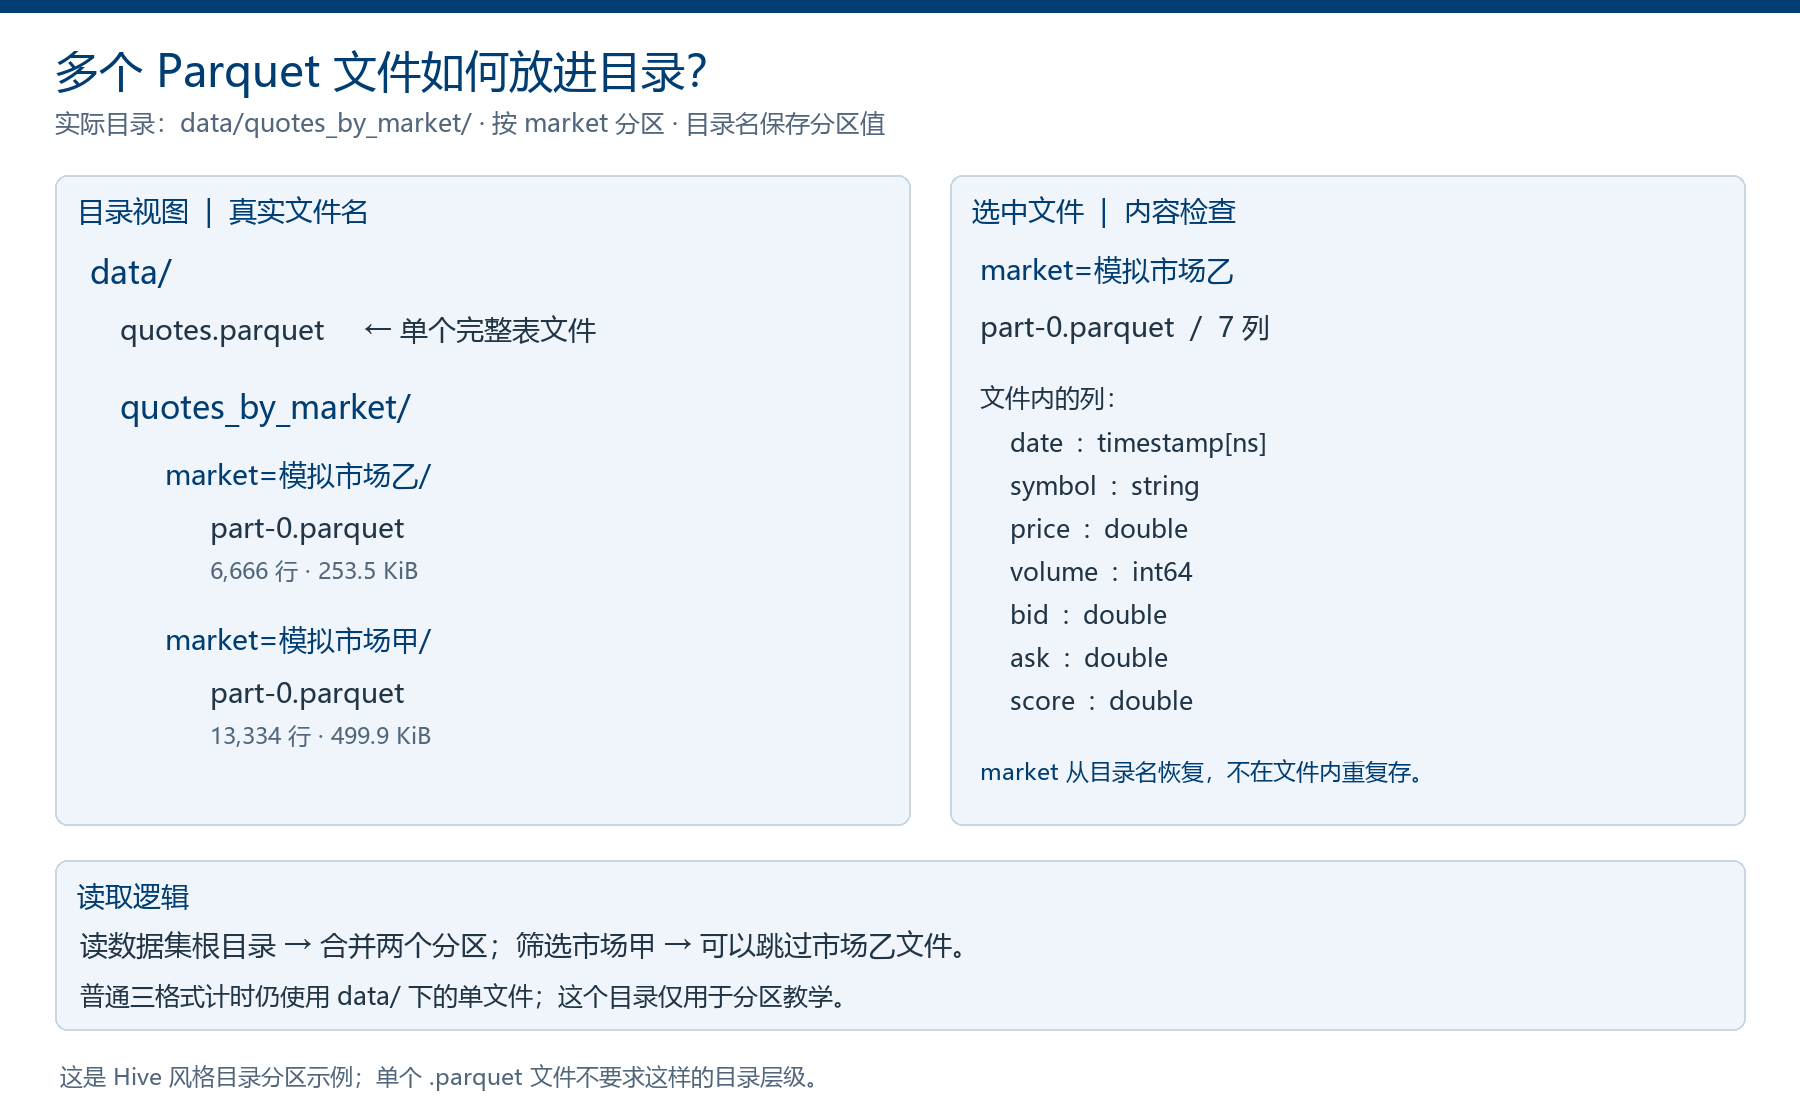
\includegraphics[width=\textwidth,height=.78\textheight,keepaspectratio]{parquet_directory.png}
\end{frame}

\begin{frame}[fragile]{读取一个文件，或读取整个分区目录}
\begin{lstlisting}
# 单个文件
one = pd.read_parquet(DATA / "quotes.parquet")
# 两个市场分区，合起来仍是同一张表
all_markets = pd.read_parquet(DATA / "quotes_by_market")
# 根据目录名，跳过另一个市场的文件
market_a = pd.read_parquet(DATA / "quotes_by_market",
    engine="pyarrow", filters=[("market", "==", "模拟市场甲")])
\end{lstlisting}
\begin{itemize}
\item \texttt{market=值} 是目录分区；行组在文件内部，不是文件夹。
\item 本例分区列从目录名恢复；读回后行顺序和分类类型可能变化。
\item 分区示例只解释组织方式，不混入三种单文件的速度比较。
\end{itemize}
\end{frame}

\begin{frame}[fragile]{Parquet 读写与类型信息}
\begin{lstlisting}
quotes.to_parquet(DATA / "quotes.parquet", index=False,
                  engine="pyarrow", compression="snappy",
                  row_group_size=5000)
back = pd.read_parquet(DATA / "quotes.parquet",
                       engine="pyarrow")
back.dtypes
\end{lstlisting}
\begin{itemize}
\item 本例日期、字符串代码和数值类型随模式保存。
\item 20,000 行按每组 5,000 行写入，得到 4 个行组。
\item \texttt{index=False} 表示不额外保存索引；需要的索引应转成列。
\item 压缩降低体积但需要解压；速度依赖数据和具体配置。
\end{itemize}
\end{frame}

\begin{frame}[fragile]{读取时选列，与读完再切列}
\begin{lstlisting}
# 读取时只要两列
small = pd.read_parquet(DATA / "quotes.parquet",
                        engine="pyarrow",
                        columns=["price", "volume"])
# 对照：先读取整表，再保留两列
wide = pd.read_parquet(DATA / "quotes.parquet", engine="pyarrow")
small_after = wide[["price", "volume"]]
\end{lstlisting}
\begin{itemize}
\item 两者返回相同内容，读取和解码的工作量却可能不同。
\item 列很多、只取少数列时，通常更值得在读取时指定列。
\item 小文件中初始化成本可能更明显，必须用实测检查。
\end{itemize}
\end{frame}

\begin{frame}[fragile]{条件筛选：返回更少行，不保证少读所有块}
\begin{lstlisting}
selected = pd.read_parquet(DATA / "quotes.parquet",
    engine="pyarrow", columns=["symbol", "price"],
    filters=[("symbol", "==", "000001")])
\end{lstlisting}
\begin{itemize}
\item pyarrow 执行条件筛选；条件允许时，统计信息帮助跳过行组。
\item 若每个行组都含目标代码，可能无法跳过任何行组。
\item 分区目录可帮助跳过文件；本章同时提供两市场的分区示例。
\item Parquet 不提供 Excel 的工作表或数据库的逐行更新接口。
\item 本章修改后重写文件；大数据集可通过增加分区文件扩展。
\end{itemize}
\end{frame}

\section{同源数据的读取速度实验}

\begin{frame}{计时之前：确认读回内容一致}
\begin{enumerate}
\item 同一张原始表、同样行数、同样列顺序，不混用过滤前后数据。
\item 检查日期类型与精度、证券代码前导零、缺失位置。
\item 浮点数采用合理容差，不要求文本往返逐位相等。
\item 验证通过后才比较速度；不能把“漏读了内容”当成提速。
\end{enumerate}
\begin{block}{Notebook 的核对方法}
先统一日期精度和字符串表示，再使用\\
\texttt{pd.testing.assert\_frame\_equal(..., check\_exact=False,}\\
\texttt{rtol=1e-9, atol=1e-8)}。\\
标准化与断言在计时外完成；读取参数的解析成本在计时内。
\end{block}
\end{frame}

\begin{frame}{实验设计：回答一个明确的问题}
\begin{itemize}
\item 问题：同一份 20,000 行 $\times$ 8 列数据，完整读成 DataFrame 要多久？
\item 生成、写入与验证不计时；计时包围一次读取调用。
\item 先预读，再重复 5 轮；每轮随机调整三种格式的顺序。
\item 保存每次耗时，报告中位数、最小值、最大值与文件体积。
\item 记录 Python、pandas、pyarrow、openpyxl 与操作系统版本。
\end{itemize}
\begin{alertblock}{明确实验边界}
未清空操作系统缓存，是有缓存条件下的端到端读取实验；不是磁盘带宽或冷启动测试，也没有测量峰值内存。
\end{alertblock}
\end{frame}

\begin{frame}[fragile]{perf\_counter：只给读取过程计时}
\begin{lstlisting}
from time import perf_counter
start = perf_counter()
back = pd.read_parquet(DATA / "quotes.parquet", engine="pyarrow")
elapsed_ms = (perf_counter() - start) * 1000
print(elapsed_ms)
\end{lstlisting}
\begin{itemize}
\item 不把打印、生成、写文件或一致性断言放进计时区间。
\item 单次波动大，Notebook 将三种读取器放入同一重复计时函数。
\item 每次得到完整 DataFrame 后再停止计时，随后释放结果。
\item 耗时用毫秒，文件体积用 KiB（1024 字节）。
\end{itemize}
\end{frame}

\begin{frame}{如何读实验表，而不是背排名}
\begin{itemize}
\item Notebook 输出：格式、中位数、最小值、最大值、文件体积。
\item 哪个最快？哪个最小？耗时波动是否会影响你的判断？
\item CSV 本例不压缩；xlsx 容器有压缩；Parquet 用 Snappy。
\item 因此比较的是这些常用配置，不是只改变“按行或按列”。
\item 不填固定的“实测大小”或通用排名：以本次运行结果为准。
\end{itemize}
\begin{block}{第二组实验：只需要价格与成交量}
比较 CSV 的 \texttt{usecols}、Parquet 的 \texttt{columns}、Parquet 全表后切列。先确认相同结果，再重复计时。
\end{block}
\end{frame}

\begin{frame}{速度差异从哪里来？}
\begin{itemize}
\item 文本格式需要将字符解析为数字、日期与缺失值。
\item Excel 还要解释工作簿和单元格结构。
\item Parquet 需要读元数据、解码与解压；选列可减少工作量。
\item 小文件可能由初始化开销主导；宽表的选列收益可能更明显。
\item 缓存、硬件、引擎、压缩、数据类型和重复率都会改变结果。
\end{itemize}
\begin{alertblock}{结论写法}
写“在这台机器、这份数据和这组参数下……”。不要写“二进制永远更快”或“某格式永远最小”。
\end{alertblock}
\end{frame}

\section{综合案例与练习}

\begin{frame}[fragile]{真实行情：计算一次，保存后复用}
\begin{lstlisting}
raw = pd.read_csv(DATA / "eod_data.csv", index_col=0,
                  parse_dates=True).dropna(subset=["SPY"])
rets = np.log(raw / raw.shift(1))
vol = (rets["SPY"].rolling(21).std() * np.sqrt(252)).dropna()
table = vol.rename("vol21").rename_axis("date").reset_index()
table.to_parquet(DATA / "spy_vol21.parquet", index=False)
table.to_excel(DATA / "spy_vol21.xlsx", index=False)
\end{lstlisting}
\begin{itemize}
\item 日期索引显式转成列，让输出结构清楚。
\item Parquet 保存中间表，Excel 提供给人工查看。
\item Notebook 随后读回并验证：保存成功还要核对内容。
\end{itemize}
\end{frame}

\begin{frame}{课堂练习与课后任务}
\begin{enumerate}
\item 预览三种文件的前 6 行，找到第一条记录和缺失值的表达方式。
\item 去掉 CSV 的 \texttt{dtype}，观察代码前导零与日期类型。
\item 用一个 ExcelWriter 写两个工作表，读回并打印表名。
\item 对 2,000 行和 20,000 行分别重做实验，记录环境、体积和耗时。
\item 选做：增加 20 个数值列，再比较 Parquet 全表与选两列。
\item 选做：将第6章的 beta 表分别保存为 CSV 与 Parquet，读回核对。
\end{enumerate}
\begin{block}{回答时至少包含}
任务是什么、数据有多大、参数是什么、结果如何、结论适用到哪里。
\end{block}
\end{frame}

\begin{frame}{本章小结：格式会影响操作方式}
\begin{itemize}
\item CSV：文本交换，明确编码和类型；选列、分块控制工作量。
\item Excel：以工作表组织，多个表共用一个 Writer。
\item Parquet：列式、类型与压缩；在读取时指定列和筛选条件。
\item 先验证数据一致，再用重复计时比较，不预设通用冠军。
\end{itemize}
\begin{exampleblock}{下章预告}
本章比较“读数据”；下一章比较“算数据”：循环、向量化与性能测量。
\end{exampleblock}
\end{frame}

\begin{frame}{参考资料与实验入口}
\small
\begin{itemize}
\item 配套 Notebook：\texttt{notebooks/07\_Input\_Output.ipynb}
\item 数据生成脚本：\texttt{scripts/prepare\_data.py}
\item 教材基础：第9章\citep{hilpisch2018python}；新增 API 参照官方文档。
\item \href{https://pandas.pydata.org/docs/reference/api/pandas.read_csv.html}{pandas：read\_csv}
\item \href{https://pandas.pydata.org/docs/reference/api/pandas.ExcelWriter.html}{pandas：ExcelWriter}
\item \href{https://pandas.pydata.org/docs/reference/api/pandas.read_parquet.html}{pandas：read\_parquet}
\item \href{https://parquet.apache.org/docs/overview/}{Apache Parquet：Overview} 与
\href{https://parquet.apache.org/docs/file-format/}{File Format}
\end{itemize}
官方文档查阅日期：2026-09-24。实验排名由本地运行产生。
\end{frame}


\appendix

\begin{frame}[allowframebreaks]{参考文献}
	\bibliographystyle{style/gbt7714-2005}
	\bibliography{reference.bib}
\end{frame}

\begin{frame}
	\begin{center}
		{\Huge\calligra Thanks for your attention!}
		\vspace{1cm}

		{\Huge Q \& A}
	\end{center}
\end{frame}

\end{document}
